\documentclass[12pt]{article}
\usepackage{amsmath}
\usepackage{amsthm}
\usepackage{tgtermes}
\usepackage{newtxmath}
\renewcommand{\familydefault}{\rmdefault}
\usepackage[L7x,T1]{fontenc}
\usepackage[utf8]{inputenc}
\usepackage[a4paper]{geometry}
\geometry{verbose,tmargin=2cm,bmargin=2cm,lmargin=3cm,rmargin=1.5cm}
\usepackage{fancyhdr}
\pagestyle{fancy}
\usepackage{color}
\usepackage[english, lithuanian]{babel}
\usepackage{booktabs}
\usepackage{enumitem}
\usepackage{cancel}
\usepackage{graphicx}
\usepackage{setspace}
\usepackage{amsmath}

\onehalfspacing
\usepackage[unicode=true,pdfusetitle,
 bookmarks=true,bookmarksnumbered=true,bookmarksopen=false,
 breaklinks=false,pdfborder={0 0 1},backref=false,colorlinks=false]
 {hyperref}
\hypersetup{
 pdfstartview=FitH, bookmarksopen=true, hidelinks=true,  pdfdisplaydoctitle=true, pdfpagemode=UseNone}

\makeatletter

%%%%%%%%%%%%%%%%%%%%%%%%%%%%%% LyX specific LaTeX commands.
\providecommand{\LyX}{\texorpdfstring%
  {L\kern-.1667em\lower.25em\hbox{Y}\kern-.125emX\@}
  {LyX}}
%% Because html converters don't know tabularnewline
\providecommand{\tabularnewline}{\\}

%%%%%%%%%%%%%%%%%%%%%%%%%%%%%% Textclass specific LaTeX commands.
\newlength{\lyxlabelwidth}      % auxiliary length 

\@ifundefined{date}{}{\date{}}
%%%%%%%%%%%%%%%%%%%%%%%%%%%%%% User specified LaTeX commands.
% Dokumento autoriai Jevgenij Chmeliov ir Andrius Gelžinis, (c) 2018
\usepackage{tocloft}
\usepackage{indentfirst}
\frenchspacing
\usepackage{cite}
\usepackage{upgreek}
\usepackage{siunitx} % dydžių vienetams
\sisetup{
output-decimal-marker = {,},
exponent-product = \cdot,
inter-unit-product = \ensuremath{\cdot} }

\usepackage[labelsep=space]{caption}
\captionsetup[figure]{name=Fig., labelsep=space}
\captionsetup[table]{name=Table, labelsep=space}
\usepackage{float}


% \usepackage[labelsep=space]{caption}
% \DeclareCaptionLabelFormat{pav}{#2~#1}
% \captionsetup[figure]{labelformat=pav, name=pav.}
% \captionsetup[table]{labelformat=pav, name=lentelė.}

\DeclareMathOperator{\Real}{Re}
\DeclareMathOperator{\Imag}{Im}
\DeclareMathOperator{\gradient}{grad}
\DeclareMathOperator{\divergence}{div}
\DeclareMathOperator{\rotor}{rot}
\DeclareMathOperator{\trace}{Tr}

\renewcommand{\headrulewidth}{0pt}
\renewcommand{\figurename}{Fig.}

\newcommand\mpl{M_{\rm pl}}

\makeatother

\begin{document}
\global\long\def\imath{\mathrm{i}}%
 
\global\long\def\ddiff{\mathrm{d}}%
 
\global\long\def\d{\mathrm{d}}%
 
\global\long\def\vect#1{\mathbf{#1}}%
 
\global\long\def\oper#1{\hat{#1}}%
 
\global\long\def\emath{\mathrm{e}}%
 

\global\long\def\ket#1{\left|#1\right\rangle }%
\global\long\def\bra#1{\left\langle #1\right|}%
\global\long\def\braket#1#2{\left\langle #1\middle|#2\right\rangle }%
 
\global\long\def\braketop#1#2#3{\left\langle #1\middle|#2\middle|#3\right\rangle }%
\global\long\def\si#1#2{\SI{#1}{#2}}%


\rhead{}

\lhead{}

\cfoot{\thepage}

\normalfont
\selectlanguage{lithuanian}
\thispagestyle{empty}
\begin{center}
Vilniaus universitetas\\
Fizikos fakultetas\\
Teorinės fizikos ir astronomijos institutas
\par\end{center}

\vspace{3.5cm}

\begin{center}
Gytis Vėjelis
\par\end{center}

\begin{center}
\textbf{The formation of primordial black holes due to resonant processes during cosmic inflation}\vspace{0.8cm}
\par\end{center}

\begin{center}
MAGISTRANTŪROS STUDIJŲ MOKSLO TIRIAMOSIOS PRAKTIKOS ATASKAITA
\par\end{center}

\begin{center}
\vspace{0.8cm}
Teorinės fizikos ir asrtofizikos studijų programa
\par\end{center}

\begin{center}
\vspace{3.5cm}
\par\end{center}

\begin{tabular*}{0.9\textwidth}{@{\extracolsep{\fill}}ll}
Studentas & Gytis Vėjelis\tabularnewline[0.5cm]
Darbo vadovas & dr. Mindaugas Karčiauskas\tabularnewline[0.5cm]
Instituto direktorius & prof. Darius Abramavičius\tabularnewline
\end{tabular*}
\begin{center}
\vfill{}
\par\end{center}

\begin{center}
Vilnius 2026
\par\end{center}

\newpage{}
\selectlanguage{english}
\normalfont\tableofcontents{}

\newpage{}

\addcontentsline{toc}{section}{Santrauka}

% \begin{center}
% \textbf{\large{}Pirminių juodųjų skylių susidarymas dėl rezonansinių procesų kosminės infliacijos metu}{\large\par}
% \par\end{center}

% \begin{center}
% \textbf{Gytis Vėjelis}
% \par\end{center}

% \begin{center}
% \textbf{Santrauka}
% \par\end{center}

% Šiame darbe nagrinėjama ankstyvosios Visatos dinamika infliacijos epochoje, ypatingą dėmesį skiriant rezonansiniams procesams, kurie gali turėti reikšmę pirminių juodųjų skylių (PJS) susidarymui. Kosmologija tiria Visatą ir jos raidą didžiausiu įmanomu masteliu. Šiuolaikinė kosmologinė paradigma remiasi dviem pagrindinėmis teorijomis: bendrąja reliatyvumo teorija (BRT), aprašančia erdvėlaikio geometriją bei gravitaciją, ir kvantine lauko teorija (KLT), kuri yra būtina dalelių fizikai ir laukų dinamikai ankstyvojoje Visatoje.

% Darbo pradžioje aptariami pagrindiniai kosmologijos principai, tokie kaip homogeniškumo ir izotropiškumo prielaidos, leidžiančios Visatos metriką aprašyti Friedmanno Lemaître’o Robertsono Walkerio (FLRW) metrika. Iš jos gaunamos Friedmanno lygtys, kurios nusako Visatos plėtimosi greitį ir pagreitį per energijos tankį $\rho$ bei slėgį $p$. Infliacija apibrėžiama kaip ankstyvasis Visatos spartaus pagreitinto plėtimosi etapas. Tokia būsena natūraliai atsiranda, jei Visatos energijos tankį dominuoja skaliarinis laukas $\phi$ (inflatonas) su potencialu $V(\phi)$.

% Infliacijos dinamikai aprašyti naudojamas Klein–Gordono tipo judėjimo dėsnis besiplečiančiame fone:
% \begin{equation*}
%     \ddot{\phi} + 3 H \dot{\phi} + V_{, \phi} = 0,
% \end{equation*}

% čia $H$ yra Hablo parametras. Įvedami pagrindiniai infliaciją apibūdinantys parametrai: $\epsilon$ ir $\eta$. Parametras
% \begin{equation*}
%     \epsilon = -\frac{\dot{H}}{H^2}
% \end{equation*}

% leidžia sekti inflacijos evoliuciją. Infliacijos pabaiga apibrėžiama $\epsilon = 1$. Darbe taip pat aptariami du svarbūs ribiniai rėžimai: lėto riedėjimo (slow-roll) ir kinacijos (kination). Lėto riedėjimo atveju kinetinė energija yra daug mažesnė už potencinę, todėl laukas juda lėtai ir palaiko ilgalaikę infliaciją. Kinacijos rėžime kinetinė energija dominuoja, o energijos tankis mažėja labai greitai ($\rho_{\phi} \propto a^{-6}$)

% Toliau darbe pereinama prie laikotarpio po infliacijos, angliškai vadinamu reheating (peršildymu). Infliacijai pasibaigus inflatonas pradeda osciliuoti aplink potencialo minimumą (arba simetrijos lūžio tašką), o jo energija perduodama kitoms dalelėms. Tai veda prie reliatyvistinės plazmos susidarymo ir radiacinės Visatos stadijos. Aptariamas perturbatyvus dalelių gamybos mechanizmas, kai inflatono skilimas aprašomas naudojant $\Gamma$ faktorių, ir peršildymo pabaiga apytiksliai nustatoma su $H ~ \Gamma$. Taip pat pristatomas ankstyvojo prieš-peršildymo modelis, kai inflatonas sąveikauja su papildomu skaliariniu lauku $\chi$ per sąveikos narį $\frac{1}{2}g^2 \phi^2 \chi^2$.

% Svarbi darbo dalis skirta parametriniam rezonansui, kuris laikomas pagrindiniu peršildymo ``varikliu''. Iš kvantuoto lauko $\chi_k(t)$ judėjimo lygčių, tam tikrose aproksimacijose gaunama Mathieu lygtis, kurios sprendinių stabilumo juostos nusako, kada lauko svyravimai yra nestabilūs ir rezonensiniai. Šiame darbe stabilumo ir nestabilumo sritys buvo apskaičiuotos Floquet teorijos metodais, o gautos rezonansinės juostos pateiktos grafiškai (stabilumo kreivės $(A_k,q)$ plokštumoje). Be to, nagrinėjamas dalelių užimtumo skaičius $n_k$, kuris leidžia stebėti dalelių gamybos stiprėjimą skirtinguose $k$-modose. Pateikiami keli skirtingų $k$ reikšmių pavyzdžiai, parodantys, kad rezonansas yra labai priklausomas nuo impulso, kai kuriuose rėžimuose dalelių gamyba vyksta "šuoliais", o kitur yra silpnesnė arba beveik nevyksta.

% Kadangi dauguma aptariamų judėjimo lygčių neturi paprastų analitinių sprendinių, darbe akcentuojamas skaitinis modeliavimas. Naudotas ketvirtos eilės Runge–Kutta (RK4) metodas, kuris pasižymi geru tikslumo ir paprastumo balansu. Parodoma, kaip antros eilės diferencialinės lygtys perrašomos į pirmos eilės sistemą įvedant pagalbinį kintamąjį $v = \dot{x}$. Tai leidžia tiesiogiai taikyti RK4 integravimo schemą.

% Rezultatų dalyje pristatomas tiriamas teorinis modelis, kuriame be inflatono $\phi$ įtraukiamas kompleksinis skaliarinis laukas $\psi$, turintis masės narį, priklausantį nuo $\phi$, ir savisąveiką $\lambda |\psi|^4$. Kompleksinis laukas išskaidomas į radialinę ir kampinę dalis $\chi$ ir $\theta$, kas leidžia gauti atskiras judėjimo lygtis šioms lauko komponentėms bei išvesti dalelių skaičiaus tankio evoliuciją. Taip pat aptariamas Hartree–Fock aproksimacijos taikymas, kai netiesiniai nariai pakeičiami vidurkiais, pvz. $\chi^3 \rightarrow 3 \langle \chi^2 \rangle \chi$, kas supaprastina skaitinį sprendimą inhomogeniškiems laukams.

% Praktinei analizei pradžioje pasirenkamas supaprastintas atvejis – nagrinėjama tik inflatono dinamika, laikant $\langle \chi \rangle = \langle \theta \rangle = 0$. Inflatonui naudojamas specifinis potencialas

% \begin{equation*}
%     V(\phi) = V_0 \exp \left[ - \kappa \exp \left( \frac{\phi}{b \mpl} \right) \right]
% \end{equation*}

% kuris pasižymi beveik plokščia sritimi mažoms $\phi$ reikšmėms ir staigiu kritimu tam tikrame intervale. Tokia forma yra svarbi, nes plokščias potencialas leidžia palaikyti lieto riedėjimo infliaciją, o staigus kritimas lemia greitą infliacijos pabaigą. Darbe pateikiamas šio potencialo grafikas, sugeneruotas skaitiniu būdu.

% Taip pat analitiškai išvedamas lieto riedėjimo sprendinys $\phi(N)$ kai laikas pakeičiamas e-foldų skaičiumi $N = \ln a$. Tai suteikia paprastą atskaitos tašką skaitinių rezultatų patikrinimui. Be to, aptariamas kinacijos režimas ir parodoma, kad šiuo atveju sprendinys artėja prie atraktoriaus

% \begin{equation*}
%     \phi(N) = \phi_* \pm \sqrt{6} (N - N_*)
% \end{equation*}

% Skaitinių skaičiavimų dalyje pateikiama integravimo strategija: pradinės sąlygos parenkamos lėto riedėjimo režime, tuomet sistema integruojama iki infliacijos pabaigos ($\epsilon = 1$). Gautuose rezultatuose matyti, kad inflatono laukas $\phi(N)$ auga sparčiai, o infliacija baigiasi ties $N_{\rm pabaiga} \approx 12.59$. Kadangi supaprastintame modelyje neįtraukti energijos nuostoliai į kitus laukus, inflatono dinamika po infliacijos tampa ``neapribota`` (nėra efektyvios trinties). Pateikiamas ir dalelių gamybos indikatorius $\ln n_k$, kuris rodo augimą su ``šuoliška'' struktūra. Pažymima, kad tokie šuoliai ir laikini kritimai nebūtinai reiškia fizinį dalelių naikinimą – tai gali būti komovinių kintamųjų ir pasirinktos $n_k$ definicijos pasekmė.

% Darbo pabaigoje pateikiamos išvados ir darbo rezultatai:
% \begin{itemize}
%     \item buvo ištirtos infliacijos judėjimo lygtys pasirinktam potencialui,
%     \item sukurta skaitinė RK4 integravimo programa,
%     \item gauti rezultatai dera su lėto riedėjimo ir kinacijos ribiniais atvejais, o pilnam modelio realizmui būtina įtraukti $\chi$ ir $\theta$ laukus, jų vidurkius bei korekcijas (pvz., 2PI), kad būtų galima aprašyti backreaction ir reheating fiziką.
% \end{itemize}

% Apibendrinant, šis darbas sukuria teorinį ir skaitinį pagrindą tolesniems tyrimams, kuriuose rezonansiniai procesai infliacijos ir preheating metu gali sustiprinti fluktuacijas ir potencialiai prisidėti prie pirminių juodųjų skylių susidarymo scenarijų analizės.

\section*{Santrauka}

Šiame darbe nagrinėjama ankstyvosios Visatos dinamika infliacijos epochoje ir po jos, ypatingą dėmesį skiriant rezonansiniams procesams, kurie gali sustiprinti laukų fluktuacijas ir sudaryti sąlygas pirminių juodųjų skylių (PJS) susidarymui. Kosmologija, siekia aprašyti Visatos raidą didžiausiais masteliais, tačiau standartinis didžiojo sprogimo palieka daug neatsakytų klausimų. Dėl šių trūkumų kosminės infliacijos teorija buvo pasiūlyta. Nūdien, kosmologija yra labai pažengus, tačiau vis dar nėra gerų paaiškinimų tamsiajai materijai, tamsiajai energijai ir kitiems fenomenams.

Darbe taikomos homogeniškumo ir izotropiškumo prielaidos, leidžiančios Visatos metriką aprašyti kaip idealaus skysčio, neturinčio vidinės trinties, dinamiką, besiplečiančiame fone. Tiksliau, infliacijos dinamika aprašoma skaliariniu lauku $\phi$ (inflatonu), judančiu savo potenciale $V(\phi)$. Šiame darbe nagrinėjamas konkretus potencialas

\begin{equation*}
V(\phi)=V_0\exp\!\left[-\kappa\exp\!\left(\frac{\phi}{bM_{\rm Pl}}\right)\right],
\end{equation*}
kuris pasižymi beveik plokščia sritimi mažoms $\phi$ reikšmėms ir staigiu kritimu tam tikrame intervale. Tokia forma yra svarbi, nes plokščias potencialas palaiko lėto-riedėjimo (slow-roll) infliaciją, o staigus kritimas lemia greitą infliacijos pabaigą ir perėjimą į kitą dinamikos režimą. Infliacijai apibūdinti įvedami standartiniai parametrai $\epsilon$ ir $\eta$, o infliacijos pabaiga apibrėžiama sąlyga $\epsilon=1$. Taip pat aptariami du ribiniai režimai: lėto riedėjimo režimas, kai potencinė energija dominuoja kinetinę, ir kinacijos (kination) režimas, kai kinetinė energija tampa svarbiausia ir inflatono energijos tankis mažėja kaip $\rho_\phi \propto a^{-6}$. Šie ribiniai atvejai naudojami kaip analitiniai orientyrai skaitiniams rezultatams patikrinti.

Toliau darbe nagrinėjamas laikotarpis po infliacijos, vadinamas reheating (peršildymu), kurio metu inflatono energija perduodama kitoms dalelių rūšims ir susidaro karšta reliatyvistinė plazma, užtikrinanti perėjimą į spinduliuotės dominuojamą Visatos stadiją. Pabrėžiama, kad ankstyvoji
peršildymo stadija (preheating) dažnai vyksta neperturbatyviai, todėl ją būtina analizuoti atskirai. Preheating metu dalelių kūrimasis gali būti itin intensyvus dėl parametrinio rezonanso: dėl osciliuojančio inflatono foninio lauko kitų laukų efektyvioji masė tampa laiko atžvilgiu periodiška,
o judėjimo lygtys įgauna parametrinio osciliatoriaus formą. Tam tikrose aproksimacijose gaunama Mathieu lygtis, kurios stabilumo ir nestabilumo juostos nusako, kuriuose parametrų režimuose lauko Fourier modai auga eksponentiškai. Šiame darbe rezonansinės sritys apskaičiuojamos Floquet teorijos metodais, o rezultatai pateikiami stabilumo diagramose $(A_k,q)$ plokštumoje. Papildomai nagrinėjamas dalelių užimtumo skaičius $n_k$, leidžiantis stebėti dalelių gamybos stiprėjimą skirtinguose impulsų $k$-moduose.

Darbo dalis skirta pirminių juodųjų skylių susidarymo idėjai. PJS gali formuotis ankstyvojoje Visatoje, jei tam tikruose masteliuose susidaro pakankamai didelės tankio pertubacijos. Infliacijos metu kvantinės fluktuacijos yra ištempiamos iki kosmologinių mastelių, o vėliau jos virsta kreivumo ir tankio netolygumais. Jei pertubacija yra pakankamai didelė, jai iš naujo įėjus į horizontą spinduliuotės dominavimo epochoje, slėgis nebesugeba sustabdyti gravitacinio kolapso ir gali susiformuoti juodoji skylė. Darbe pateikiama metrikos pertubacijų analizė Niutono kalibravimo sąlyga (Newtonian gauge), išvedamos perturbuotos lauko lygtys Fourier erdvėje ir parodoma, kaip iš sprendinių galima apskaičiuoti pirminių kreivumo pertubacijų galios spektrą $P_\zeta(k)$. Aptariama, kad
stebėjimams suderintas modelis turi būti beveik mastelio invariantinis kosminės foninės spinduliuotės masteliuose, tačiau mažesniuose masteliuose galios spektras turi sustiprėti, kad būtų įmanomas PJS
formavimasis.

Kadangi dauguma aptariamų diferencialinių lygčių neturi paprastų analitinių sprendinių, darbe akcentuojamas skaitinis modeliavimas. Naudotas ketvirtos eilės Runge-Kutta (RK4) metodas, kuris pasižymi geru tikslumo ir paprastumo balansu. Parodoma, kaip antros eilės differencialinės lygtys perrašomos į pirmos eilės sistemą įvedant pagalbinį kintamąjį, todėl galima tiesiogiai taikyti RK4 integravimo schemą. Rezultatų dalyje pristatomas tiriamas teorinis modelis, kuriame be inflatono $\phi$ įtraukiamas kompleksinis skaliarinis laukas $\psi$, turintis $\phi$ priklausantį masės narį ir savisąveiką $\lambda|\psi|^4$. Kompleksinis laukas išskaidomas į radialinę ir kampinę dalis $\chi$ ir $\theta$, išvedamos atskiros judėjimo lygtys šioms komponentėms bei dalelių skaičiaus tankio evoliucija per Noether srovę. Taip pat aptariamas Hartree-Fock aproksimacijos taikymas, kai netiesiniai nariai pakeičiami vidurkiais, kas supaprastina inhomogeniškų laukų skaitinį sprendimą.

Kosminės infliacijos metu galima laikyti, kad $\langle\chi\rangle=\langle\theta\rangle=0$. Tai leidžia patikimai nustatyti infliacijos pabaigą ir patikrinti, kad skaitiniai sprendiniai dera su lėto riedėjimo ir kinacijos ribiniais atvejais. Skaitiniai rezultatai rodo, kad inflatono laukas $\phi(N)$ sparčiai auga, o infliacija baigiasi ties $N_{\rm end}\approx 12.59$, kai $\epsilon=1$. Taip pat pateikiamas dalelių skaičius $\ln n_k$, kuriame matomas augimas su charakteristine struktūra. Aptariama, bendra kompiuterinio algoritmo strategija, naudota išspręsti dabartines lygtis ir kaip šį algoritmą būtų galima taikyti toliau, norint įtraukti vėlesnes Visatos raidos epochas. 

Apibendrinant, šiame darbe nagrinėtas kosminės infliacijos modelis:
išanalizuota pirmąją Visatos epochą šiame modelyje. Sukurtas teorinis ir skaitinis pagrindas tolesniems tyrimams, kuriuose rezonansiniai procesai infliacijos ir preheating metu gali sustiprinti fluktuacijas ir potencialiai prisidėti prie pirminių juodųjų skylių susidarymo scenarijų analizės.


\section{Introduction}

Cosmology is the study of the Universe as a whole. How does the Universe evolve? What are the physical laws that shape its large scale structures? For most of the human history nobody knew the answers to these questions. The Universe was thought to be static, eternal, unchanging \cite{palmer2008parmenides}. Even the existence of other galaxies is a relatively modern discovery \cite{hubble1925cepheids}. During the twentieth century these questions got new answers. New observations and physical theories showed that the Universe is not in fact static. This history of the Universe implied that the Universe looked very different than it does now.  

The idea that the Universe is expanding was one of the first major revolutions \cite{hubble1929relation}. Once this expansion was established, it became natural to imagine rewinding cosmic history. If space is stretching today, then the Universe must have been more compressed, meaning denser and hotter in the past. This reasoning gave rise to the Hot Big Bang framework \cite{alpher1948origin}, which successfully explains many observed features of the cosmos, including the abundance of light elements and the existence of the cosmic microwave background radiation.

However, as cosmology matured into a precision science, it became clear that the standard Big Bang picture leaves important questions unanswered. Why does the Universe look so similar in all directions, even across regions that seem too far apart to have ever been in contact? Why is the geometry of space so close to flat? And where did the tiny initial irregularities come from that later grew into galaxies?

In response to the apparent limitations of the Hot Big Bang (HBB) model, the theory of cosmic inflation was proposed. Today it plays a central part in cosmological research. With growing interest in the field, inflationary cosmology has had major developments and thus various theories alongside many observations \cite{levi2019dark} \cite{aghanim2020planck}. This raises a challenge: a successful theory not only has to be mathematically correct, but also fit the known observations and hopefully provide additional explanations for dark energy, dark matter, baryogenesis or other phenomena. One of the theories will be investigated in this work.

The goal of this work is to investigate the inflaton field equations of motion with numerical methods and obtain numerical solutions of inflaton field for the $V(\phi) = V_0 \exp ( - \kappa \exp(\frac{\phi}{b M_{\rm pl}})) $ potential. With the aim to apply the results obtained later to a more diffuclut equations of coupled fields.

In the following work natural units will be used $c=\hbar=1$.

\subsection{Cosmology and Inflation}

Cosmology aims to investigate the Universe on the largest scales. It requires the best known theories of physics, namely, Einstein's General Relativity (GR) \cite{carroll2019spacetime} and Quantum Field Theory \cite{zee2010quantum}. The former describes the dynamics of spacetime using the Einstein's field equations

\begin{equation}\label{eq: einsteins field equations}
    G_{\mu \nu} = 8 \pi G T_{\mu \nu},
\end{equation}
where $G_{\mu \nu}$ is the Einstein tensor, $T_{\mu \nu}$ is the energy-momentum tensor and $G$ is the Newton's gravitational constant. This relation provoked the well known quote by John Archibald Wheeler "Spacetime tells matter how to move; matter tells spacetime how to curve." This is because the Einstein tensor depends on the spacetime metric, while the energy-momentum tensor describes the energy distribution of the system. In addition, there are several symmetries which one can take advantage of when deriving the equation. In the study of cosmology two main assumptions are made: first, that on sufficiently large scales the Universe is homogeneous (though some recent investigations start to question this assumption \cite{simpson2025beyond}) and secondly, that it is isotropic. Furthermore, we know that the Universe is expanding, hence the spacetime geometry is well described by the Friedmann Lemaître Robertson Walker (FLRW) metric \cite{friedmann1922125}

\begin{equation}
    ds^2 = - dt^2 + a(t)^2 \left[ \frac{dr^2}{1-kr^2} + r^2 (d \theta^2 + \sin^2 \theta \d \phi^2) \right],
\end{equation}
where $a(t)$ is the scale factor for the expanding Universe, $k \in \{ 0, +1, -1 \}$ determines the spatial curvature (flat space, positive curvature and negative curvature accordingly). Assuming isotropic space, spherical coordinate system was used. In addition, assuming homogeneous space, the Universe can be modeled as a perfect fluid with $T^{\mu \nu} = \mathrm{diag}(\rho, p, p,p)$, where  $p$ is pressure and $\rho$ is the energy density. The dynamics of this fluid in an expanding background is described by the Friedmann equations

\begin{align}
    H^2 &\equiv \left( \frac{\dot{a}}{a} \right)^2 = \frac{8 \pi G}{3} \rho - \frac{k}{a^2}, \label{eq: Friedmann equation} \\
    \frac{\ddot{a}}{a} &= -\frac{4 \pi G}{3} (\rho + 3 p) \label{eq: acceleration equation},
\end{align}
here $H(t)$ is the Hubble parameter. Observations indicate that the Universe had an accelerated expansion in the early Universe, which we call inflation. During this period the Universe had to have negative pressure and a quasi-exponential growth in the scale factor

\begin{equation}
    a(t) \propto \exp(Ht), \qquad \ddot{a}>0 \quad \text {with} \quad \rho + 3p<0.
\end{equation}

There are several problems in cosmology such as the flatness problem and the horizon problem \cite{dimopoulos2020introduction}. Inflation not only offers solutions to these problems, but also has a possibility of describing baryogenesis (matter creation in the early Universe) and a possible solution to dark matter. The details of these explanations highly depend on the choice of inflation mechanisms. In many models, inflation is described by the spin-0 scalar field $\phi$ called the inflaton field that roll down the potential $V(\phi)$. The evolution of the field can then be derived using the aforementioned quantum field theory. The action in general is given by

\begin{equation}
    S = \int d^4 x \sqrt{-g} \left[ \frac{\mpl^2}{2}R - \frac{1}{2} g^{\mu \nu} \partial_{\mu} \phi \partial_{\nu} \phi - V(\phi) \right],
\end{equation}
where $\mpl = (8 \pi G)^{-1/2}$ often taken to be 1. After varying the action with respect to the metric $g_{\mu \nu}$ we reobtain the equations (\ref{eq: einsteins field equations}) and by varying $\phi$ we get the Klein-Gordon equation in an expanding background \cite{kofman1997towards}

\begin{eqnarray}
    \ddot{\phi} + 3H \dot{\phi} + V_{, \phi}(\phi) = 0.
\end{eqnarray}
There are several useful parameters that describe inflation. We can define $\epsilon$ as the background expansion parameter:

\begin{equation}
    \epsilon \equiv - \frac{\dot{H}}{H^2}.
\end{equation}
Then inflation happens when $\ddot{a} > 0 $, which implies that $\epsilon < 1$, analagously we can state that inflation ends when $\epsilon = 1$ and using

\begin{equation}
    \epsilon = \frac{\dot{\phi}^2}{2 \mpl^2 H^2}
\end{equation}
we can compute the $\dot{\phi}$ at the end of inflation. In addition, there is the Hubble flow parameter $\eta$ defined as

\begin{equation}
    \eta \equiv \frac{\dot{\epsilon}}{H \epsilon}.
\end{equation}
This parameter measures how fast $\epsilon$ changes. Often, the models for inflation are too difficult to solve analytically, hence numerical simulations are used. However, it still useful to analyse limiting cases, for several reasons. First, analytic solutions in some regime might give a way to check wheather numerical calculations are correct and coincide in some range. Secondly, analytic solutions often give physical insights that numerical solutions can not provide. There are two popular limits concerning the evolution of the inflaton field. Slow-roll inflation happens at the beggining of inflation. This approximation happens when the field rolls so slowly that we can neglect the kinetic term, meaning $\frac{1}{2} \dot{\phi}^2 \ll V(\phi)$. This now gives the justification as to why there was negative pressure and why it caused accelerated expansion. Using the spacial part of the energy-momentum tensor, taking the slow-roll limit and equation (\ref{eq: acceleration equation})

\begin{equation}
    p = \frac{1}{2} \dot{\phi} - V(\phi) \quad \Rightarrow \quad p \approx -V \quad \Rightarrow \quad \ddot{a} > 0
\end{equation}
Additionaly, in this limit, the Friedmann equations (\ref{eq: Friedmann equation}) and (\ref{eq: acceleration equation}) simplify to

\begin{equation}
    H^2 \approx \frac{V(\phi)}{3 \mpl^2} \quad \text{and} \quad 3 H \dot{\phi} = - V^{\prime}(\phi),
\end{equation}
where the slow-roll requires that $\epsilon \ll 1$ and $\eta \ll 1$ \cite{kofman1994reheating}. These conditions often simplify the equations enough, so that analytic solutions could be obtained. While slow-roll approximation gives the approximation for the slow evolution of inflaton field, conversely kination acts in the opposite regime. After inflation, we can also investigate the regime where the kinetic energy of the field dominates the potential, meaning $\frac{1}{2} \dot{\phi}^2 \gg V(\phi)$, then

\begin{eqnarray}
    \rho_{\phi} \approx \frac{1}{2} \dot{\phi}^2 \qquad \text{and} \qquad p_{\phi} \approx \frac{1}{2} \dot{\phi}^2.
\end{eqnarray}
With a negligible $V^{\prime}(\phi)$, the equation of motion for the inflaton field then becomes very simple

\begin{equation}
    \ddot{\phi} + 3 H \dot{\phi} \approx 0.
\end{equation}
Which implies that $\dot{\phi} \propto a^{-3}$ and $\rho_{\phi} \propto a^{-6}$, which is a much faster dilution of energy density than that of the matter or radiation fluids.

Thus far we have not considered any coupling to the inflton field. Additional massive spinnor fields must be added to model to model the decay of the inflaton field into particles in order to reproduce the Universe we see today. It will be shown that the inflaton field, through the process of preheating and reheating, decays into these spinor fields.

\subsection{Reheating and Preheating}

It can be shown that the temperature of the thermal bath filling the Universe decreases with the expansion of the Universe $T \propto \frac{1}{a}$ \cite{dimopoulos2020introduction}. Thus the early Universe is not only dense, but also very hot. After the rapid expansion which occurs during inflation the Universe enters a phase called reheating. The energy stored in the inflaton field decays and turns into a hot plasma of relativistic particles. These particles can be considered as radiation as they are extremely relativistic (for massive particles $E \gg m$). This gives the explanation of why the Universe after inflation is radiation dominated and thermalised.

At the end of inflation the inflaton field $\phi$ begins to oscillate around the minimum of $V(\phi)$. It should be noted, however, that in this work an alternative approach is considered - oscillation around a symmetry breaking point. As the inflaton oscillates it excites other fields, transfering energy to them and decreasing oscillating amplitude. More concretely, consider the potential $V(\phi) = \frac{1}{2}m^2(\phi - \sigma)^2$, where $\sigma$ is the minimum of the potential. Shifting $\phi - \sigma \rightarrow \phi$ leads to symmetry breaking, and we get interaction terms for scalar field $\chi$ and spinor field $\psi$
\begin{equation}
    \mathcal{L}_{\rm int} = -g^2 \sigma \phi \chi - h \bar{\psi} \psi \phi
\end{equation}
which eventually leads to inflaton decays

\begin{equation}
    \Gamma(\phi \rightarrow \chi \chi) = \frac{g^4 \sigma^2}{8 \pi m} \quad \text{and} \quad \Gamma(\phi \rightarrow \bar{\psi} \psi) = \frac{h^2 m }{8 \pi}
\end{equation}
In addition, it can be shown that during this time the inflaton field oscillates as $\phi(t) \approx \Phi(t) \sin (mt)$. Finally, it is possible to obtain the Boltzmann equation for the number density $n_{\phi}$ and energy density $\rho_{\phi}$

\begin{equation}
    \frac{d}{dt} (a^3 n_{\phi}) = -a^3 n_{\phi} \Gamma \quad \text{and} \quad \frac{d}{dt} (a^3 \rho_{\phi}) = - \Gamma a^3 \rho_{\phi}
\end{equation}
which shows that that the comoving number density of $\phi$ particles, together with the energy density of the field exponetnially decays with the rate $\Gamma$. Reheating finishes roughly at $H ~ \Gamma$, giving $T_r \approx 0.2 \sqrt{\Gamma \mpl}$. 

The early stages of reheating, called preheating, are non-pertubative and thus require different analytical methods.

The early part of reheating, called preheating, can be analysed seperately, as it involves non-pertubative dynamics. Particle production during preheating comes from nonlinear resonant instabilities in equations with parametric resonance. Continuing our discussion of reheating, we can also look at the evolution of the matter field $\chi$. After quantisation we obtain that each Fourier mode $\chi_k(t)$ must satisfy:

\begin{eqnarray}
    \ddot{\chi}_k + 3 \frac{\dot{a}}{a}\dot{\chi}_k + \left( \frac{k^2}{a^2} + m_{\chi} + g^2 \phi^2 \right) \chi = 0.
\end{eqnarray}
Due to time depensence of $\phi(t)$, this equation basically describes a harmonic oscillator with variable frequency, otherwise known as paramatric oscillator. Since the field makes so many oscillations over one Hubble time, we can neglect the expansion of the Universe. Take $a=1$ and after rearranging some terms and using the solution for the inflaton field we obtain the Mathieu equation

\begin{equation}
    \chi_k^{\prime \prime} + (A_k - 2 q \cos 2 z) \chi_k = 0
\end{equation}
where $A_k = \frac{k^2}{m^2} + 2q$ and $q = \frac{g^2 \Phi^2}{4 m^2}$. Equations with periodic forcing terms are analysed with Floquet theory \cite{brown2012floquet}, and in the case of Mathieu's equations stability/instability bands were computed in this work.

% \begin{center}
%     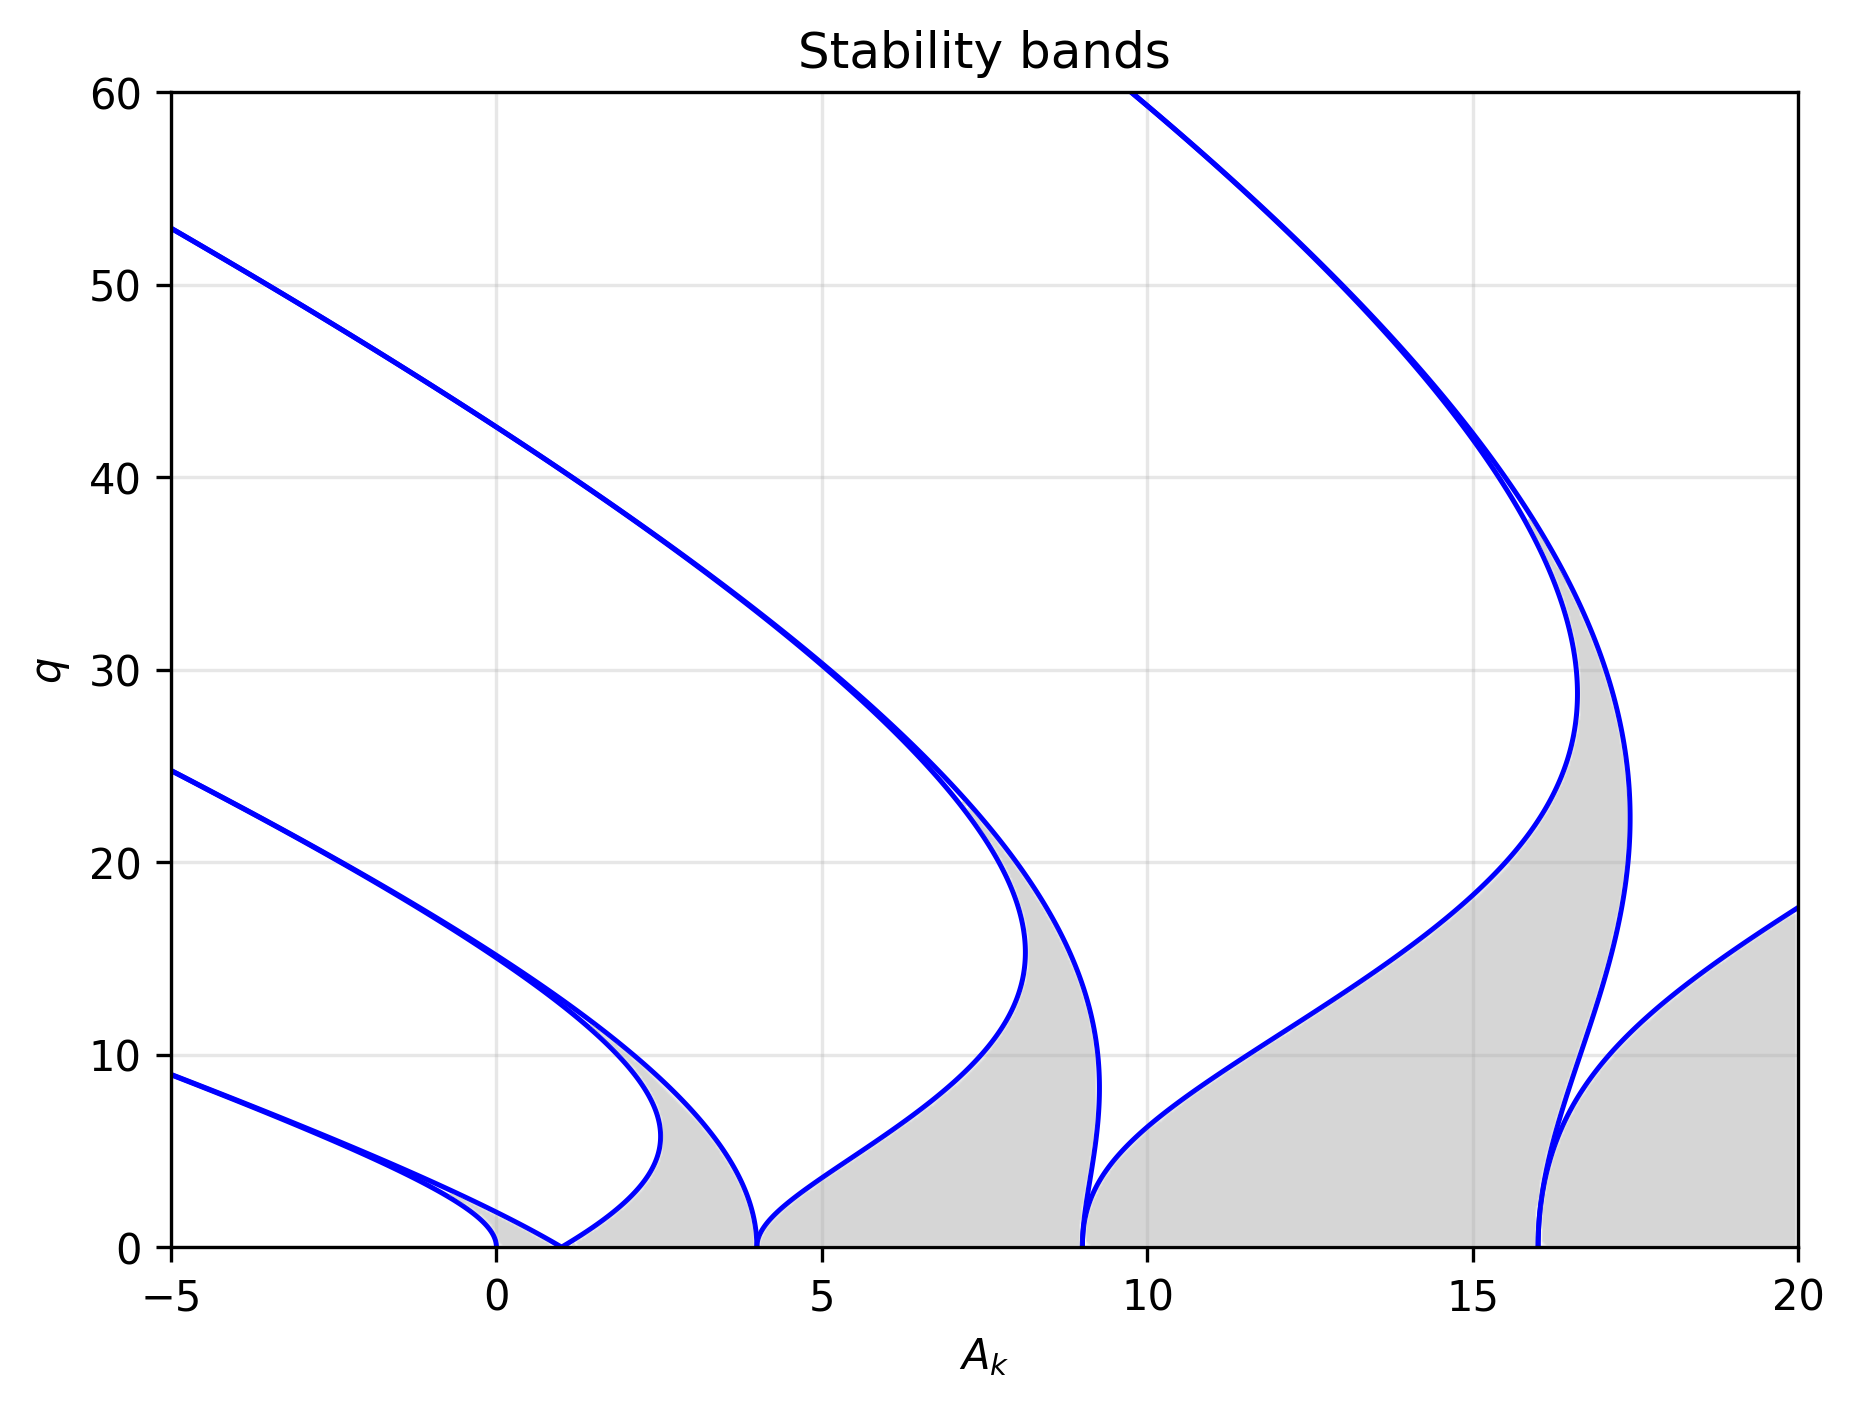
\includegraphics[width=300pt]{images/matheius_curves.png}
% \end{center}

\begin{figure}[H]
    \centering
    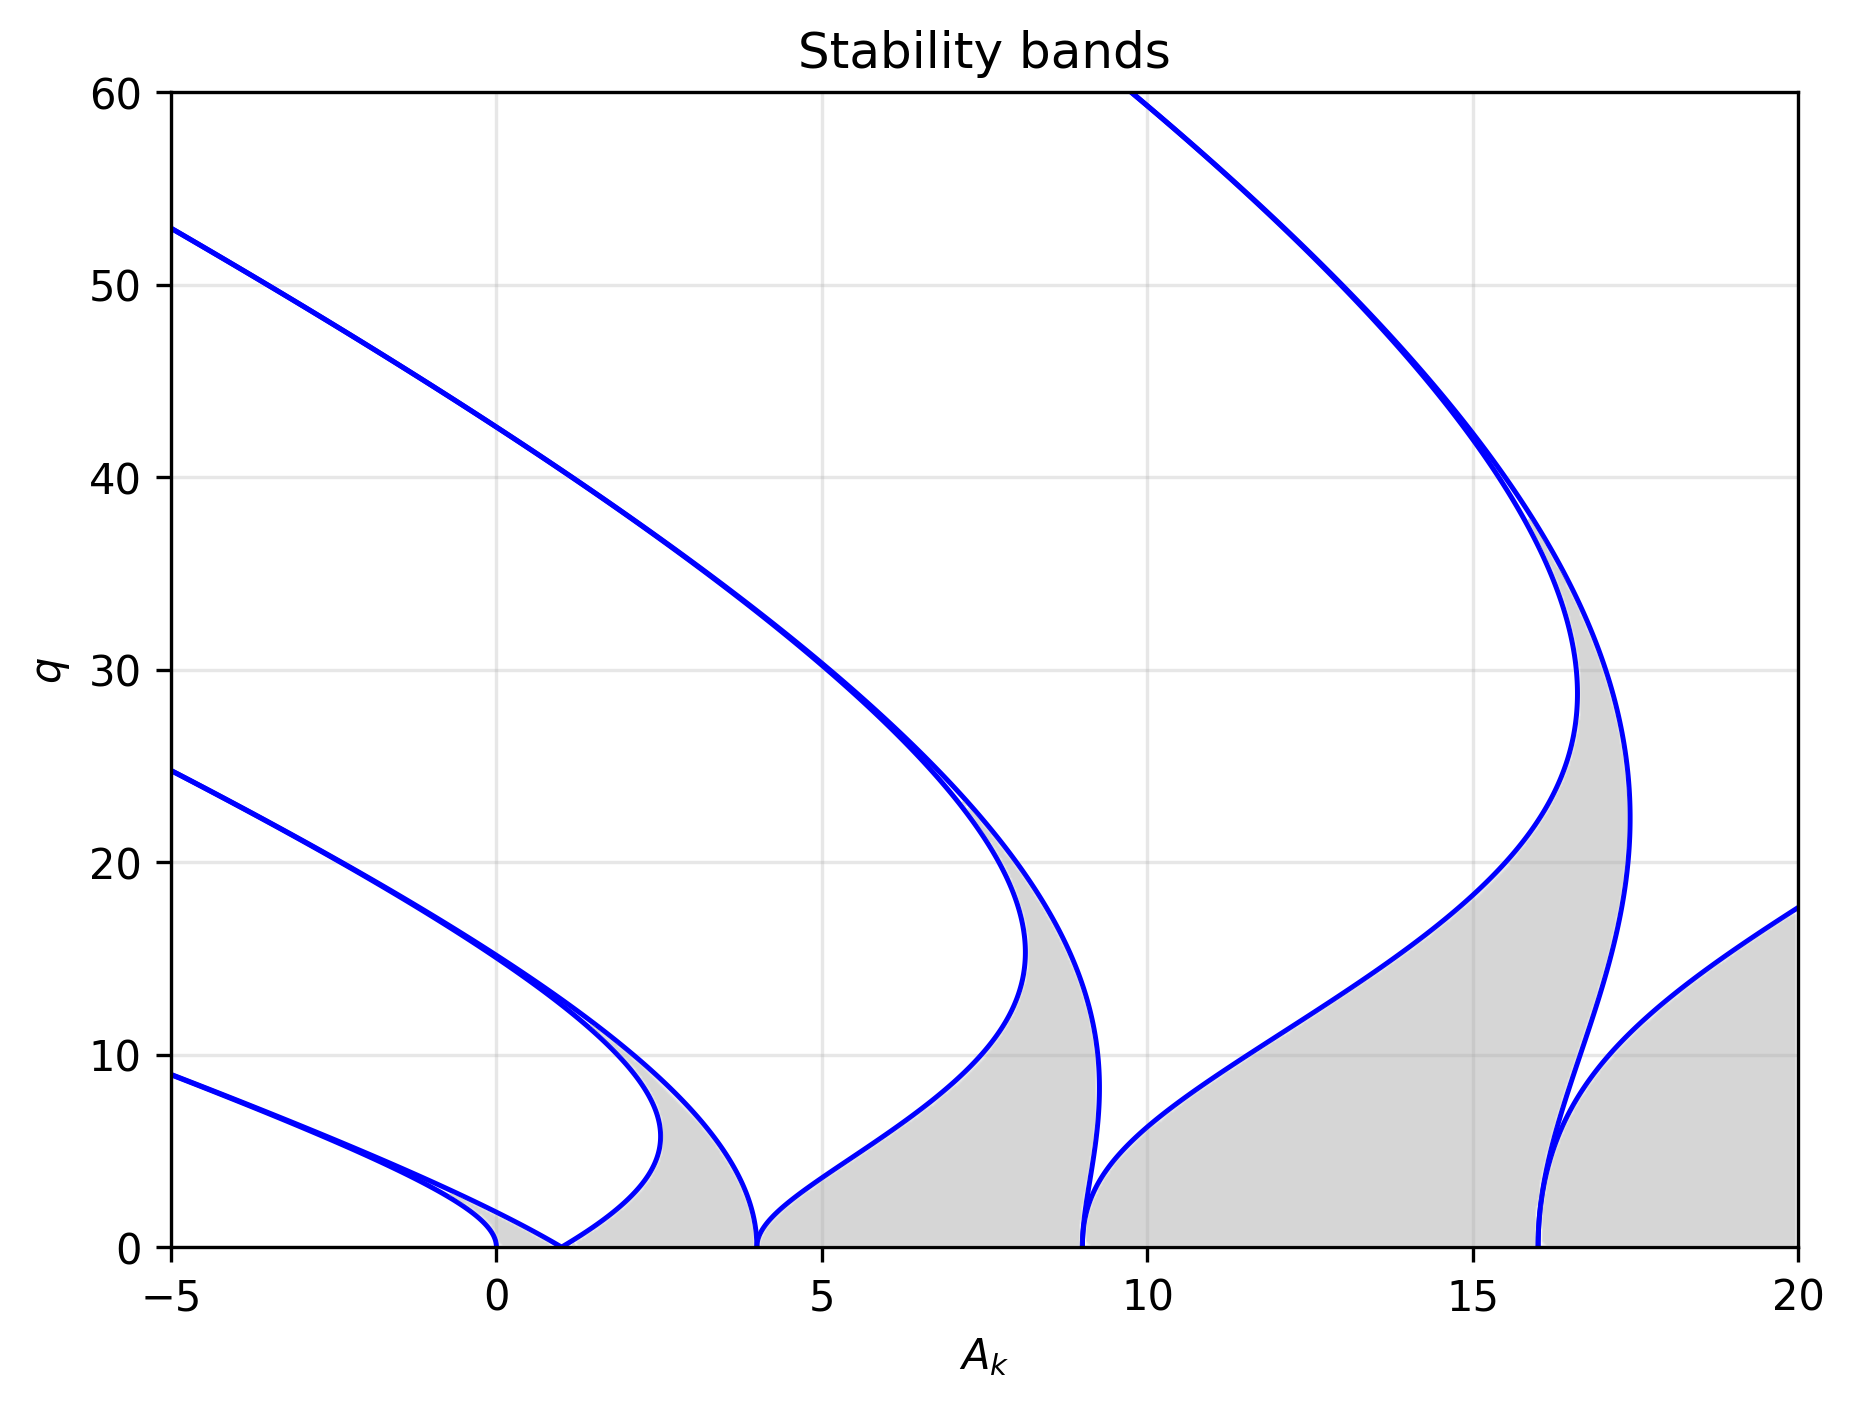
\includegraphics[width=300pt]{images/matheius_curves.png}
    \caption{Stability/instability structure of the Mathieu equation in the $(A_k,q)$ parameter plane. The blue curves mark the boundaries of the resonance bands obtained numerically in this work using Floquet analysis, showing (shaded) regions where solutions for $\chi_k$ grow exponentially (parametric resonance) versus remain bounded (unshaded).}
    \label{fig:matheius_curves}
\end{figure}

This gives us insights into parametric resonance of the $\chi$ equations of motion. Parametric resonance is often referred to as the engine of preheating. It is an explosive amplification of field fluctuations caused by the inflaton field oscillations. Since inflaton is coupled to matter fields like $\chi$, it transfers its energy and the effective mass term of the $\chi$ field becomes time dependent. Hence knowing the stability bands allows us to see where the instabilities and resonances happen. Similarly as before, we can compute the comoving occupation number of particles $n_k$ in the mode $k$ in an expanding Universe

\begin{equation}
    n_k = \frac{\omega_k}{2} \left( \frac{|\dot{\chi}|^2}{\omega_k^2} + |\chi_k|^2 \right) - \frac{1}{2}
\end{equation}
where
\begin{equation}
    \omega^2_k = \frac{k^2}{a^2(t)} + g^2 \Phi^2 \sin^2 mt + m_\chi^2 - \frac{3}{2} \left( \frac{\dot{a}}{a} \right) - \frac{3}{2} \frac{\ddot{a}}{a}
\end{equation}
Note that this function does not have any factors inversely proportional to the volume $a^3$. These factors appear when the number density of particles is calculated in non-comoving coordinates. Hence we can plot the evolution of some $k$-modes during the early stages of parametric resonance. Different Fourier $k$-modes will experience resonance differently. This can be easily seen in the following graphs

% \begin{center}
%     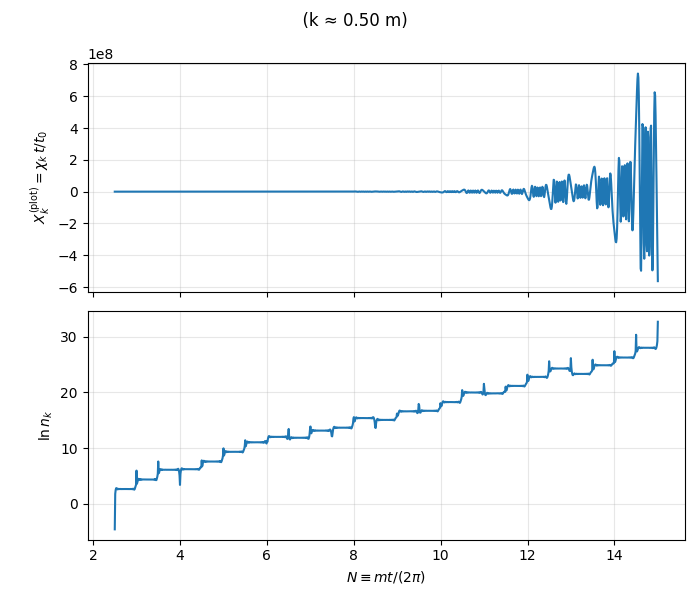
\includegraphics[width=300pt]{images/k050.png}
% \end{center}

\begin{figure}[H]
    \centering
    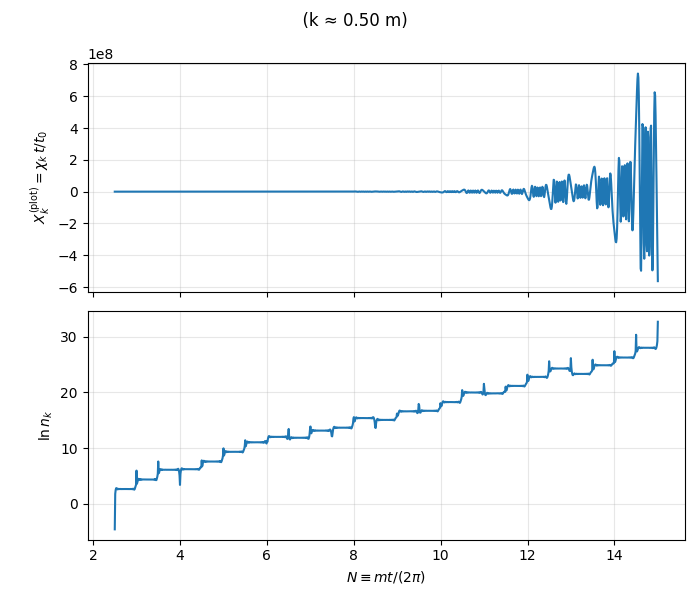
\includegraphics[width=300pt]{images/k050.png}
    \caption{Early-stage parametric resonance for the mode $k=0.50\,m$ in the simplified preheating model. Top: time evolution of the field mode $\chi_k(t)$ showing the onset of amplification driven by the oscillating inflaton background. Bottom: corresponding comoving occupation number $\ln n_k$, computed numerically in this work from the mode functions, illustrating the growth of particle production in the resonant regime.}

    \label{fig:k050}
\end{figure}

% \begin{center}
%     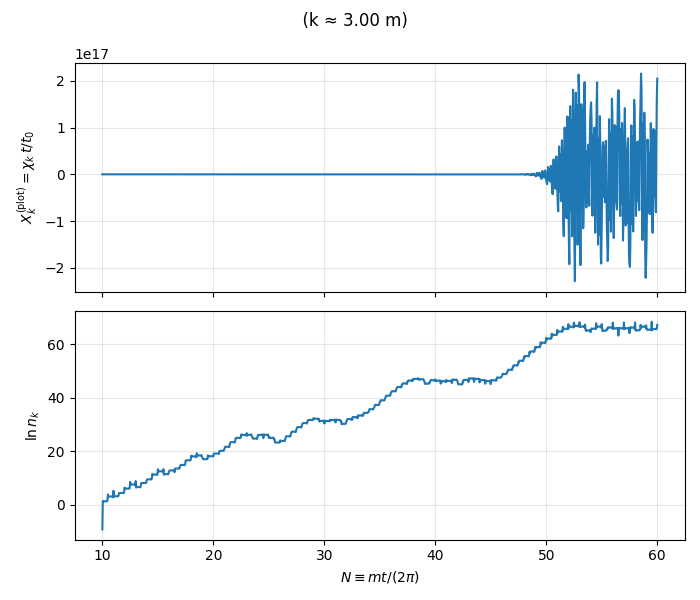
\includegraphics[width=300pt]{images/k300.png}
% \end{center}

\begin{figure}[H]
    \centering
    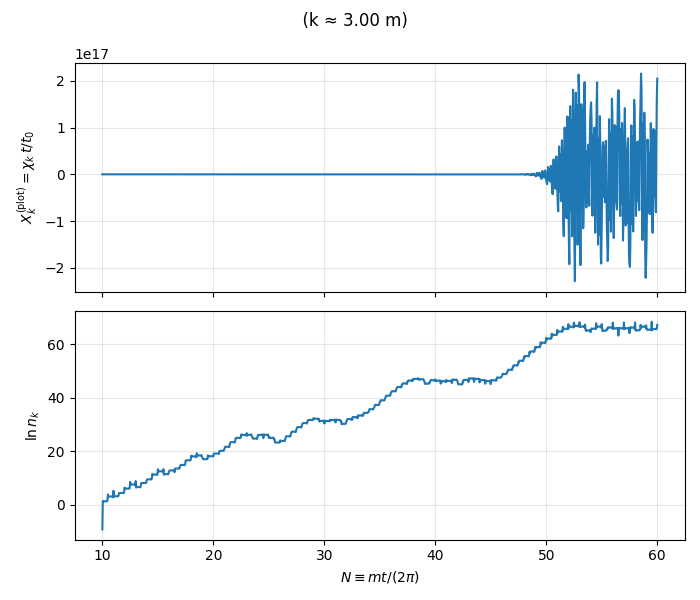
\includegraphics[width=300pt]{images/k300.png}
    \caption{Early-stage parametric resonance for the mode $k=3.00\,m$. Top: evolution of $\chi_k(t)$ exhibiting a different amplification pattern compared to smaller $k$. Bottom: numerical evolution of $\ln n_k$ obtained in this work, demonstrating mode-dependent particle production and resonance strength.}
    \label{fig:k300}
\end{figure}

% \begin{center}
%     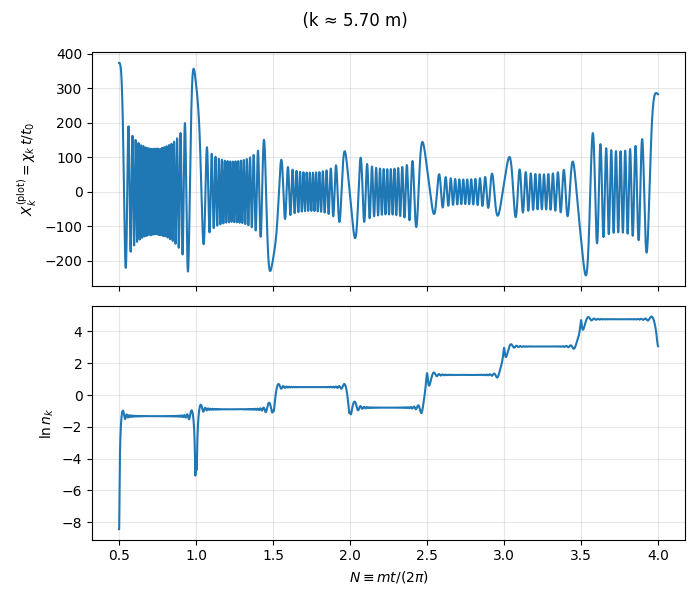
\includegraphics[width=300pt]{images/k570.png}
% \end{center}


\begin{figure}[H]
    \centering
    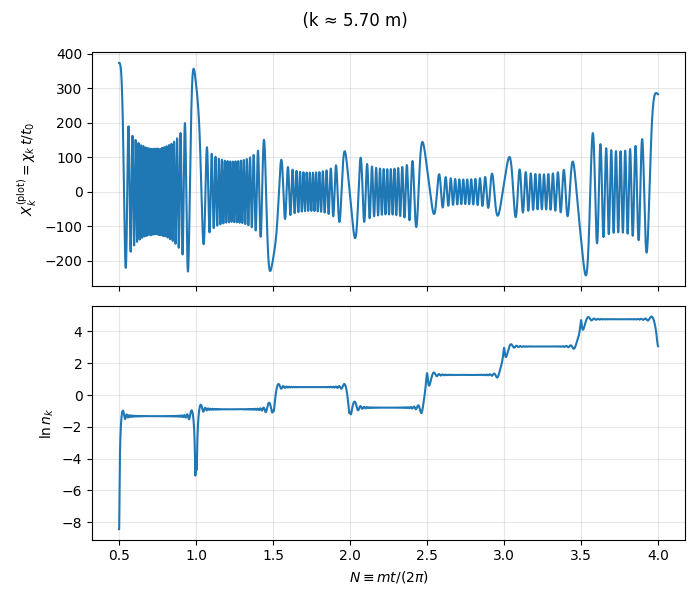
\includegraphics[width=300pt]{images/k570.png}
    \caption{Parametric resonance behaviour for the mode $k=5.70\,m$. Top: numerical solution for $\chi_k(t)$ showing oscillatory dynamics with bursts of amplification. Bottom: $\ln n_k$ computed in this work, where the step-like growth and temporary drops reflect the use of comoving variables rather than physical number density, not actual particle destruction.}
    \label{fig:k570}
\end{figure}

% \begin{figure}[H]
%     \centering
%     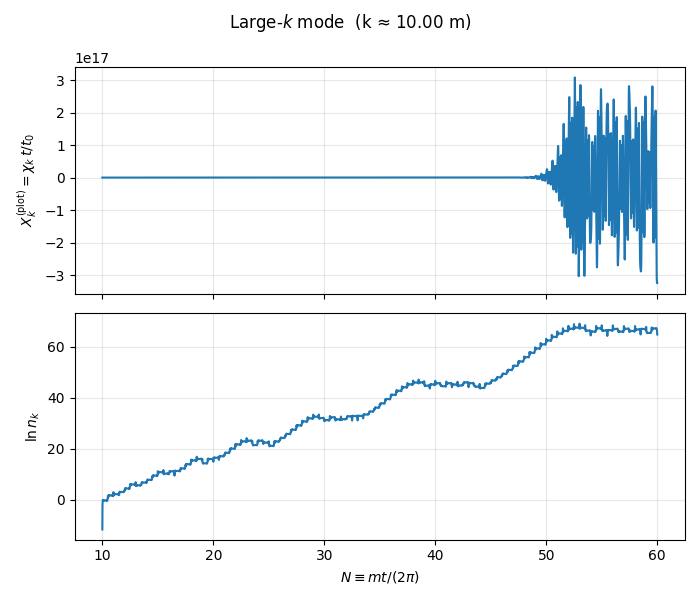
\includegraphics[width=300pt]{images/k1000.png}
%     \caption{Large-$k$ mode evolution for $k\simeq 10\,m$ obtained numerically in this work.  Top: the rescaled mode function $X_k^{(\mathrm{plot})}=\chi_k\,t/t_0$ remains small during the early evolution and then undergoes a rapid amplification at later times, indicating the onset of a resonant instability for this high-momentum mode.  Bottom: the corresponding comoving occupation number $\ln n_k$ shows an overall growth with step-like features, reflecting non-adiabatic particle production in an oscillating inflaton background; the small oscillations and plateaus are characteristic of the comoving definition of $n_k$ and do not imply physical particle destruction.}
%     \label{fig:k1000}
% \end{figure}

Notice that the particle number doesn't increase monotonically. The drops in the number of particles does not mean that the particles are being destroyed.


\subsection{Primordial black holes and pertubations of spacetime}
Primordial black holes (PBHs) are black holes that could have formed in the early Universe, long before stars and galaxies existed. Unlike astrophysical black holes, which form from stellar collapse at late times, PBHs may originate from large primordial perturbations generated in the very early Universe \cite{carr1974black}.

In inflationary cosmology, quantum fluctuations of light fields are stretched to macroscopic scales by the accelerated expansion. These fluctuations appear as perturbations of the spacetime curvature and later translate into density perturbations of the cosmic plasma. In most regions the perturbations are small and eventually lead to the formation of large scale structure, but in rare cases the perturbation amplitude might be unusually large. If such an overdense region re-enters the horizon during the radiation dominated era, exceeding some critical threshold, pressure forces would be unable to prevent gravitational collapse, and the region could form a black hole \cite{carr1974black}.

Putting this more concretely, consider the FLRW metric with a Newtonian gauge is given by \cite{karciauskas2025primordial}

\begin{equation}
    ds^2 = -(1 + 2\Phi)dt^2 + a^2(t)(1 - 2 \Phi) \delta_{ij}dx^i dx^j,
\end{equation}
where we used the Einstein summation convention, with $\delta_{ij}$ being the kronecker delta and $\Phi$ being the metric perturbation variable. Scalar fields $\phi$ and $\chi$ are also perturbed,  and assuming that the homogeneous value is much greater than the perturbations $\bar{\phi} \gg \delta \phi$ allows us to write the equations of motion for the homogeneous and perturbed components seperately. Homogeneous equations are
\begin{equation}
    \ddot{\phi} + 3H \dot{\phi} + V_{, \phi} = 0 \quad \text{and} \quad \ddot{\chi} + 3H \dot{\chi} + V_{, \chi} = 0,
\end{equation}
where the Hubble parameter is $3H^2 = \frac{1}{2}\dot{\phi}^2 + \frac{1}{2}\dot{\chi}^2 + V$. In the Newtonian gauge the perturbation equations are then
\begin{align}
\delta \ddot{\phi}_k + 3H\,\delta \dot{\phi}_k
+ \left(\frac{k^2}{a^2} + V_{,\phi\phi}\right)\delta \phi_k
&= 2\left(2\dot{\phi}\,\dot{\Phi}_k - V_{,\phi}\Phi_k\right) - V_{,\phi\chi}\delta \chi_k, \\[6pt]
\delta \ddot{\chi}_k + 3H\,\delta \dot{\chi}_k
+ \left(\frac{k^2}{a^2} + V_{,\chi\chi}\right)\delta \chi_k
&= 2\left(2\dot{\chi}\,\dot{\Phi}_k - V_{,\chi}\Phi_k\right) - V_{,\phi\chi}\delta \phi_k, \\[6pt]
\dot{\Phi}_k + H\Phi_k
&= \frac{1}{2}\left(\dot{\phi}\,\delta \phi_k + \dot{\chi}\,\delta \chi_k\right).
\end{align}
with the Einstein equation acting as a constraint equation
\begin{equation}
\left(\dot{\phi}^{2} + \chi^{2} - 2\frac{k^{2}}{a^{2}}\right)\Phi_{k}
= \dot{\phi}\,\delta\dot{\phi}_{k} + \dot{\chi}\,\delta\dot{\chi}_{k}
- \ddot{\phi}\,\delta\phi_{k} - \ddot{\chi}\,\delta\chi_{k}.
\end{equation}
Note that these equations of $\delta \phi_k$, $\delta \chi_k$ and $\Phi_k$ describe the evolution of the Fourier modes of perturbation variables $\delta \phi$, $\delta \chi$ and $\delta \Phi$ respectively. The solutions of these equations allows us to compute the power spectrum $\mathcal{P}_{\zeta}(k)$ of primordial curvature pertubations $\zeta$:
\begin{equation*}
    \mathcal{P}_{\zeta}(k) = \frac{k^3}{2 \pi^2} |\zeta_k|^2 \quad \text{where} \quad \zeta_k
= \Phi_k + 2H\,\frac{\dot{\Phi}_k + H\Phi_k\left(1+\frac{1}{3}\frac{k^2}{a^2H^2}\right)}
{\dot{\phi}^2 + \dot{\chi}^2}. 
\end{equation*}

Power spectrum gives the description of the typical size of primordial fluctuations $\zeta$ at some scale $k$. Meaning that if $\mathcal{P}_k$ is sufficiently small then the Universe is smooth, while a large $\mathcal{P}_k$ would mean a strongly perturbed space. PBHs form when perturbations on some small scale are large enough. To coincide with observations the power spectrum should be nearly scale-invariant in the order of CMB. While on small scales the power spectrum should enhance, so that sufficiently large overdensities can collapse into black holes. Depending on their abundance and mass distribution, PBHs have been studied as possible contributors to dark matter \cite{karciauskas2025primordial}.

\subsection{Numerical simulation}

In many physical and mathematical models the evolution of some system is given by a system of ordinary differential equations

\begin{equation}
    \frac{dy}{dt} = f(t,y),
\end{equation}
with some initial conditions $y(t_0) = y_0$, where $y(t)$ is the unknown function and $f(t,y)$ describes how the system changes in time. Unfortunately, many systems cannot be solved analytically, hence numerical methods are used. The idea behind these methods is that they discretise the domain of the independent variable and integrate along small steps. If the steps are small enough, then the error accumulation is negligible. In this work fourth-order Runge-Kutta method (RK4) will be used. It is one of the most popular algorithms as it provides high accuracy while remaining relatively simple to implement \cite{chapra2012applied}, \cite{butcher2016numerical}. The algorithm approximates the solution over a small step $h$ from $t_n$ to $t_{n+1} = t_n + h$ by combining slope estimates. Other, less accurate methods use slopes at the beginning of the step, thus quickly accumulating errors. RK4 on the other hand evaluates the slope at intermediate points and forms a weighted average. This provides stability and accuracy for the solution. Given the current $y_n \approx y(t_n)$, four intermediate values are computed

\begin{align}
k_1 &= f(t_n, y_n), \\
k_2 &= f\!\left(t_n+\frac{h}{2},\, y_n+\frac{h}{2}k_1\right), \\
k_3 &= f\!\left(t_n+\frac{h}{2},\, y_n+\frac{h}{2}k_2\right), \\
k_4 &= f\!\left(t_n+h,\, y_n+h k_3\right).
\end{align}

then the solution is updated as

\begin{equation}
    y_{n+1}=y_n+\frac{h}{6}\left(k_1+2k_2+2k_3+k_4\right).
\end{equation}

The fourth order of the RK4 extremely improves error rates since they are of order $\mathcal{O}(h^4)$ and the local truncation error per step is of order $\mathcal{O}(h^5)$

It should be noted that in many physical systems the equations of motion are usually second-order derivatives. They however can be viewed as a system of two ordinary differential equations

\begin{equation}
    \frac{d^2 y}{dt^2} = f(\dot{y}, y, t) \quad \Rightarrow \quad
        u = \frac{dy}{dt} \quad \text {and} \quad
        \frac{du}{dt} = f(u, y, t)
\end{equation}

These are usually written as vectors and the equations are then vectorised. In the following section we implement the above RK4 scheme to evolve the inflaton field numerically in an expanding Universe with application to a novel inflation theory \cite{dimopoulos2002modeling}.

\section{Results}

\subsection{Theoretical derivations}
In this section we summarise the equations used in our numerical implementation and present the background evolution of the inflaton in the simplified decoupled limit. Consider the Lagrangian density \cite{Apostolos}

\begin{equation}
    \mathcal{L} = \frac{1}{2} \nabla_{\mu} \phi \nabla^{\mu} \phi + \nabla_{\mu} \psi^* \nabla^{\mu} \psi - V(\phi) - \frac{1}{2} m_{\psi}^2(\phi) |\psi|^2 - \frac{\lambda}{4} |\psi|^4 - \frac{\lambda}{4}f^4,
\end{equation}
with the mass term

\begin{equation}
    m_{\psi}^2(\phi) = g^2 (\phi - \phi_{SBP})^2 - \lambda f^2,
\end{equation}
where the $\nabla_{\mu}$ denotes the covariant derivative, $\lambda$, $g$ and $f$ are free parameters. In particular $\lambda$ and $g$ are coupling constants. Here $f^4$ is the constant vacuum energy expectation value, in order to normalise the potential so that the true vacuum energy is zero \cite{dimopoulos2019quintessential}. In addition, $\phi$ is the inflaton field and $\psi$ is complex spin-0 scalar field. Finally, $\phi_{SBP}$ is the inflaton value at the symmetry-breaking point. 

% After the usual process of varying the fields we obtain the equation of motion for $\psi$

% \begin{equation}
%     \ddot{\psi} + 3H \dot{\psi} - \frac{1}{a^2} \nabla^2 \psi + \frac{\delta \mathcal{V}}{\delta \psi^{\dag}} = - \frac{\delta V}{\delta \psi^{\dag}}
% \end{equation}

% Where $\mathcal{V}$ is the potential energy density and $V$ was added as an external CP-violating potential. 

We can compute the particle number density, using Noether current, to be

\begin{equation}
    \dot{n} + 3H n = 2 \mathrm{Im} \left( \psi \frac{\delta V}{\delta \psi^{\dag}} \right)
\end{equation}
Next, we can decompose the complex scalar field in the polar form
\begin{equation}
    \psi(x,t) = \frac{1}{\sqrt{2}} \chi(x,t) e^{i \theta(x,t)},
\end{equation}
here $\chi$ is the radial (amplitude) mode and $\theta$ is the angular (phase) mode. Thus we obtain the following equations of motion

\begin{align}
\ddot{\chi} + 3H\dot{\chi}
-\left[\dot{\theta}^{\,2}-\frac{1}{a^{2}}(\nabla\theta)^{2}\right]\chi
+\frac{\delta \mathcal{V}}{\delta \chi}
&= -\,\frac{\delta V}{\delta \chi},
\\[6pt]
\ddot{\theta}
+\left[3H + 2\,\partial_{0}\ln(\chi)\right]\dot{\theta}
-\frac{1}{a^{2}}\Big[\nabla^{2}\theta + 2\,\nabla\ln(\chi)\cdot\nabla\theta\Big]
&= -\,\frac{1}{\chi^{2}}\frac{\delta V}{\delta \theta}.
\end{align}
Here $V_A$ denotes the CP-violating term responsible for charge production. Similarly, we apply the decomposition to the particle number to get

\begin{equation}
\dot{n} + 3Hn
= \frac{1}{a^{2}}\,\nabla\cdot\left(\chi^{2}\nabla\theta\right)
- 2\,\mathrm{Im}\!\left(\psi\,\frac{\delta V_A}{\delta\psi}\right).
\end{equation}

For computational results it is more useful to use the average, which is a typical result

\begin{equation}
\langle \dot{n} \rangle + 3H \langle n \rangle
= -2 \left\langle \mathrm{Im}\!\left(\psi\,\frac{\delta V_A}{\delta\psi}\right) \right\rangle .
\end{equation}

If we were to keep the fluctuations, we would have to replace the non-linear terms. Since in general $\chi(t)$ and $\theta(t)$ are inhomogeneous fields we can replace these terms using Hartree-Fock approximation

\begin{equation}
    \chi^3 \rightarrow 3 \langle \chi^2 \rangle \chi
\end{equation}
remember that $\phi$ depends on time and is homogeneous in space and more precisely is the expectation value, while $\chi$ and $\theta$ are inhomogeneous fields whose mean values vanish, $\langle \chi \rangle = \langle \theta \rangle = 0$, but with non-zero variance such as $\langle \chi^2 \rangle$. Taking $V(\phi) = V_0 \exp [- \kappa \exp(\frac{\phi}{b \mpl})]$, where $b = \sqrt{a}$ with $\kappa$ being a free parameter. $V_0$ can be obtained from observations. In particular, equations of motion in Fourier space can be derived

\begin{equation}
\ddot{\phi} + 3H \dot{\phi}
 - \frac{\kappa V_0}{b M_{\rm Pl}}
 \exp\!\left[\frac{\phi}{b M_{\rm Pl}} - \kappa e^{\frac{\phi}{b M_{\rm Pl}}}\right]
 + g^2 \langle \chi^2 \rangle (\phi - \phi_{\rm SBP}) = 0
\end{equation}

\begin{equation}
\ddot{\tilde{\chi}}_{\mathbf{k}} + 3H \dot{\tilde{\chi}}_{\mathbf{k}}
+ \left[
\frac{k^2}{a^2}
+ g^2 (\phi - \phi_{\rm SBP})^2
- \lambda f^2
+ 3 \lambda \langle \chi^2 \rangle + \langle \dot{\theta}^2 \rangle
+ \frac{1}{a^2} \langle (\nabla \theta)^2 \rangle
\right]
\tilde{\chi}_{\mathbf{k}} = 0
\end{equation}

\begin{equation}
\langle \chi^2 \rangle \ddot{\tilde{\theta}}_{\mathbf{k}}
+ (2 \langle \chi \dot{\chi} \rangle + 3H \langle \chi^2 \rangle) \dot{\tilde{\theta}}_{\mathbf{k}}
+ \frac{k^2}{a^2} \langle \chi^2 \rangle \tilde{\theta}_{\mathbf{k}} = 0
\end{equation}
where the averages are

\begin{equation}
\langle \chi^2 \rangle
= \int_{\mathbb{R}^3} \frac{d^3 p}{(2\pi)^3}
\left[ |\tilde{\chi}_{\mathbf{p}}(t)|^2 + \text{2PI-corrections} \right]
\end{equation}

\begin{equation}
\langle \dot{\theta}^2 \rangle
= \int_{\mathbb{R}^3} \frac{d^3 p}{(2\pi)^3}
\left[ |\dot{\tilde{\theta}}_{\mathbf{p}}(t)|^2 + \text{2PI-corrections} \right]
\end{equation}
here the 2PI-corrections stand for two particle irreducable corrections. These corrections account for backreaction, rescattering and thermalisation effects, which become important during preheating, especially when produced fluctuations grow large.

The shape of the potential is very important and is plotted as follows:

% \begin{center}
%     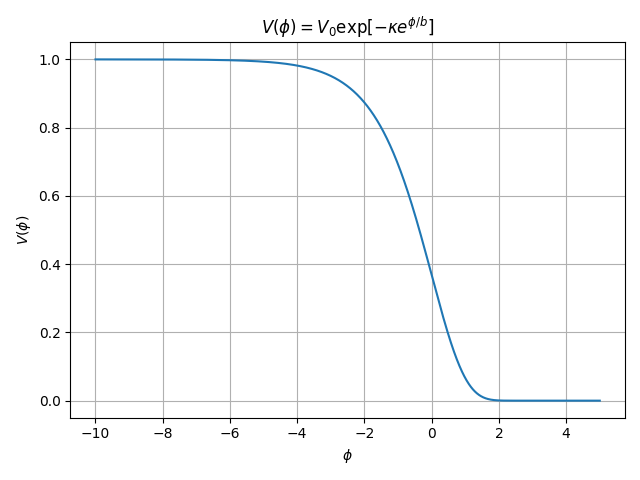
\includegraphics[width=300pt]{images/potential.png}
% \end{center}

\begin{figure}[H]
    \centering
    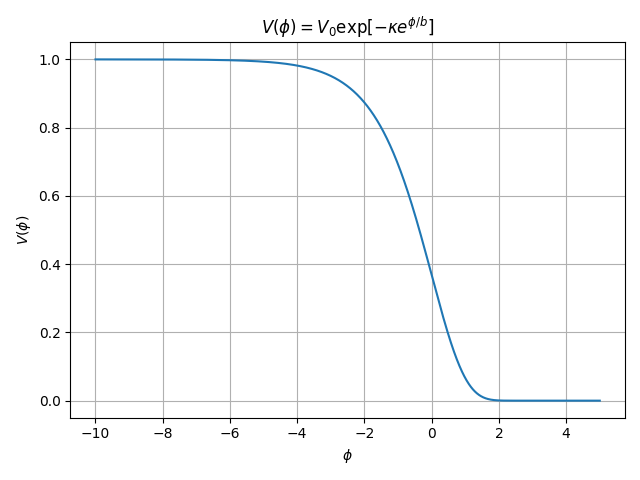
\includegraphics[width=300pt]{images/potential.png}
    \caption{Shape of the inflationary potential $V(\phi)=V_0\exp\!\left[-\kappa\exp\!\left(\phi/(bM_{\rm pl})\right)\right]$. The plot was generated in this work to illustrate the nearly flat region at small $\phi$ (supporting slow-roll inflation) followed by a rapid drop, which strongly affects the inflaton dynamics and the end of inflation.}
    \label{fig:potential}
\end{figure}


Notice that for small $\phi$, the potential is nearly flat, supporting slow-roll inflation, while at large $\phi$ it decreases rapidly, strongly affecting the end of inflation and the symmetry-breaking transition. Until it reaches some threshold and starts to rapidly fall. More importantly, this potential does not have a minimum, so an alternative mechanism of reheating is required. At around $\phi_{SBP}$, the effective mass of $\phi$ changes sign (becomes tachyonic), triggeting symmetry breaking and rapid growth. Then the inflaton can start oscillating and transfer energy to the other fields. Similar potentials, namely, exponential potential was investigated previously \cite{karvciauskas2022quintessential}, however with the release of new data, it was found that the model does not work in all regimes.

\begin{figure}[H]
    \centering
    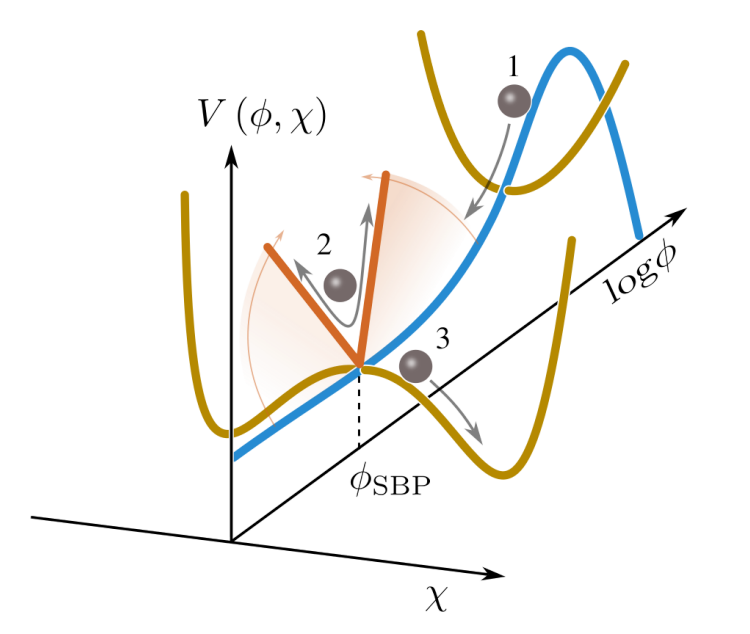
\includegraphics[width=300pt]{images/potential illustration.png}
    \caption{Illustration of the evolution of the inflaton field. After slow-roll rolling along the blue direction (stage 1), the field reaches the SBP and resonantly excites $\chi$, generating an effective linear potential and amplifying metric perturbations (stage 2). When resonance ends, the system rolls along the waterfall potential (brown) with $\phi=\phi_{\rm SBP}$. This illustration is from \cite{karciauskas2025primordial}}
    \label{fig:potential illustration}
\end{figure}

For the beginning of the project, we first take a simplified case, where we only investigate the evolution of the inflaton field. This simplification effectively describes the inflation period, during which the $\psi$ field is heavy, hence we take $\langle \chi \rangle = \langle \theta \rangle = 0$. Then the $\phi$ equations of motion are simply

\begin{equation}
    \ddot{\phi} + 3H \dot{\phi} - \frac{\kappa V_0}{b M_{\rm Pl}} \exp\!\left[\frac{\phi}{b M_{\rm Pl}} - \kappa e^{\frac{\phi}{b M_{\rm Pl}}}\right] = 0
\end{equation}
Changing the variables from time to the number of e-folds 

\begin{equation}
    t \rightarrow N, \quad \text{where} \quad N = \ln a
\end{equation}

\begin{equation}
    \dot{A} = H A^{\prime} \quad \text{and} \quad \ddot{A} = H^2 A^{\prime \prime} + H^{\prime} H A^{\prime}
\end{equation}
where the primes denote derivatives with respect to $N$. Using the Klein–Gordon equation together with the Friedmann and acceleration equations, we obtain

\begin{equation}
    \phi^{\prime \prime} + \left( 3 - \frac{{\phi^{\prime}}^2}{2 \mpl^2} \right) \phi^{\prime} + \left( 3 \mpl^2 - \frac{1}{2} {\phi^{\prime}}^2 \right) \frac{V_{, \phi}}{V} = 0
\end{equation}
Another, similar trick can be used with potential

\begin{equation}
    W = \ln V \quad \Rightarrow \quad W_{, \phi} = \frac{V_{, \phi}}{V}
\end{equation}
This is especially useful, since our potential is exponential, so using $V(\phi) = V_0 \exp \left[ - \kappa e^{\frac{\phi}{b M_{\text{Pl}}}} \right]$ we get

\begin{equation}
    W = - \kappa \exp \left( \frac{\phi}{b \mpl} \right) + W_0 \quad \text{and} \quad W_{, \phi} = -\frac{\kappa}{b \mpl} \exp \left( \frac{\phi}{b \mpl} \right)
\end{equation}
where $W_0 = \ln V_0$. Furthermore by multiplying everything by $\phi^{\prime}$, then $\phi^{\prime \prime} \phi^{\prime} = \frac{1}{2} ({\phi^{\prime}}^{2})^{\prime}$ and $W_{, \phi} \phi^{\prime} = b \mpl W^{\prime}$, hence

\begin{equation}
    ({\phi^{\prime}}^{2})^{\prime} + \left( 6 - {\phi^{\prime}}^2 \right) {\phi^{\prime}}^2 + \left( 6 - {\phi^{\prime}}^2 \right) b W^{\prime} = 0
\end{equation}
where we used $\mpl = 1$. There is also the kination limit, which was discussed a bit earlier. These equations can now be numerically simulated. Before proceeding to numerical results, approximations can also be considered. As mentioned before, we can use slow roll approximation for the beginning of inflation, when potential terms dominate kinetic terms. Consider that $|\ddot{\phi} | \ll |3 H \dot{\phi}|$ and $|\ddot{\phi} \ll |V_{, \phi} (\phi)|$, so Friedmann equation simplifies to

\begin{equation}
    H^2 = \frac{V(\phi)}{3 \mpl^2}
\end{equation}
And slow-roll Klein-Gordon equation (variables depending on time) become:
\begin{equation}
    3H \dot{\phi} = - V_{, \phi}(\phi)
\end{equation}
Again, using the same change of variables $t \rightarrow N$ we have
\begin{equation}
    3H^2 \phi^{\prime} = - V_{, \phi} \quad \Rightarrow \quad \phi^{\prime} = - \mpl^2 \frac{V_{, \phi}(\phi)}{V(\phi)} = - \mpl^2 W_{, \phi}
\end{equation}
This now is easily solvable analytically, again, setting $\mpl = 1$

\begin{align*}
    N - N_0 = \int -\frac{1}{W_{, \phi}} d\phi = \int \frac{b}{\kappa} \exp \left( - \frac{\phi}{b} \right) d \phi = -\frac{b^2}{\kappa} \exp(-\frac{\phi}{b})
\end{align*}
Finally, obtaining

\begin{equation}
    \phi(N) = - b \ln \left( \frac{\kappa}{b^2} (N_0 - N) \right) = - b \ln \left( e^{-\phi_0/b} \frac{\kappa}{b^2} - N \right)
\end{equation}

This is just a simple exponential growth, which can be seen in the following figure.

% \begin{center}
%     
\includegraphics[width=300pt]{images/slowroll.png}
% \end{center}
\begin{figure}[H]
    \centering
    
\includegraphics[width=300pt]{images/slowroll.png}
    \caption{Analytic slow-roll solution $\phi(N)$ as a function of the number of e-folds $N=\ln a$ for the exponential-to-exponential potential. This curve was plotted in this work from the derived closed-form expression and demonstrates the characteristic gradual evolution of the inflaton during the slow-roll phase.}
    \label{fig:slowroll}
\end{figure}

Conversely, kination limit can also be investigated. As mentioned before, in this limit, the kinetic terms dominate. This is a simpler problem since we can neglect the potential leaving
\begin{equation}
    \phi^{\prime \prime} + \left( 3 - \frac{\phi^{\prime 2}}{2 \mpl^2} \right)\phi^{\prime} \approx 0
\end{equation}

Solving this equation gives the attractor:
\begin{equation}
    \phi(N) = \phi_* \pm \sqrt{6} (N - N_*)
\end{equation}

with $\mpl = 1$ and the star index notation meaning, that the value of the field and e-fold number is at some reference point.

\newpage

\subsection{Numerical calculations}

To solve the dynamical system numerically, the equations of motion were first
rewritten in a first-order vector form suitable for Runge-Kutta integration.
In particular, each second-order equation of the form $\ddot{x}=F(x,\dot{x},t)$
was mapped to a coupled first-order system by introducing an auxiliary variable
$v\equiv \dot{x}$, such that
\begin{equation}
    \dot{x}=v,
    \qquad
    \dot{v}=F(x,v,t).
\end{equation}
The resulting state vector is then evolved using a fixed-step fourth-order
Runge-Kutta (RK4) method.

The numerical procedure is summarized as follows:

\begin{itemize}
    \item \textbf{Initial conditions and slow-roll start.}
    Since the initial value of $\dot{\phi}$ is not specified independently, we
    initialize the inflaton dynamics in the slow-roll regime.
    Using the slow-roll approximation, we estimate $\dot{\phi}_0$ and compute
    the initial slow-roll parameter
    \begin{equation}
        \epsilon \equiv \frac{\dot{\phi}^{2}}{2H^{2}M_{\rm Pl}^{2}},
    \end{equation}
    with $M_{\rm Pl}=1$ in geometrised units. The Hubble rate is evaluated self-consistently from the Friedmann equation \ref{eq: Friedmann equation}.

    \item \textbf{Evolution until the end of inflation.}
    Starting from the slow-roll initial conditions, the full equations of motion
    are integrated forward in time (or equivalently in e-folds $N$) until inflation
    ends, defined by the condition $\epsilon=1$. The corresponding time $t_{\rm end}$
    (or $N_{\rm end}$) is recorded.

    \item \textbf{Locating the symmetry-breaking transition.}
    During the integration we identify the symmetry-breaking point by monitoring
    the model-dependent condition for the transition (e.g.\ the vanishing of an
    effective mass term or the crossing $\phi=\phi_{\rm SB}$). This defines the
    transition time $t_{\rm SB}$ (or $N_{\rm SB}$).

    \item \textbf{Restarting the integration near the transition.}
    To resolve the dynamics around symmetry breaking with improved numerical
    stability, we restart the integration at a time slightly before the transition,
    $N_{\rm start}=N_{\rm SB}-\Delta N$, with $\Delta N$ chosen to be a small number
    of e-folds. The system is then evolved through the transition and into the
    post-inflationary regime.
\end{itemize}

Finally, the implementation was designed to be modular and scalable, allowing the model parameters, initial conditions, and numerical settings (step size, stopping conditions, and diagnostics) to be modified in a straightforward way for further development and parameter scans.

The evolution of the inflaton field is as expected, a rapid growth resembling an exponential.

% \begin{center}
%     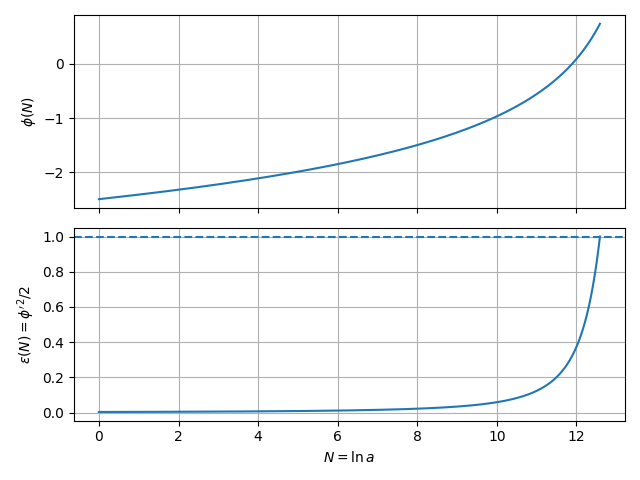
\includegraphics{images/phi evolution.png}
% \end{center}

\begin{figure}[H]
    \centering
    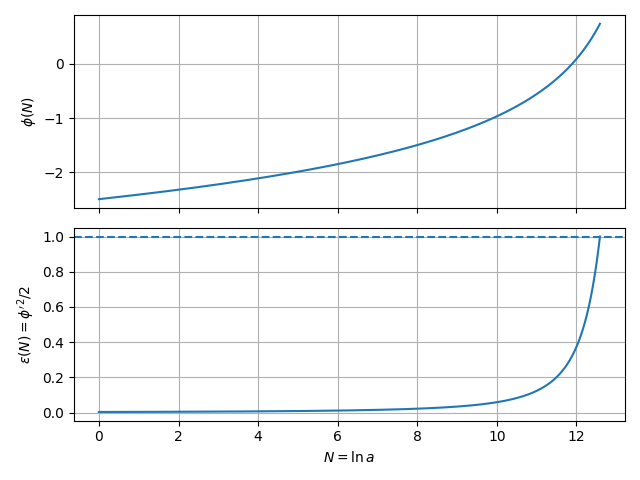
\includegraphics[width=300pt]{images/phi evolution.png}
    \caption{Numerical evolution of the inflaton field $\phi(N)$ obtained in this work using a fixed-step RK4 integrator. The solution shows the expected rapid growth in the chosen model, and inflation terminates at $N_{\rm end}\approx 12.59$ as determined by the condition $\epsilon=1$.}
    \label{fig:phievolition}
\end{figure}

In the inflaton-only approximation, the only damping is Hubble friction. Since no energy is transferred into other fields, the inflaton does not experience additional effective dissipation, and its post-inflationary evolution becomes unrealistic. $N_{\rm end} \approx 12.592333$. We verified numerical stability by repeating the integration with smaller step sizes and confirming that $N_{\rm end}$ converges. Plotting the particle number we observe a similar result as in the simplified model

% \begin{center}
%     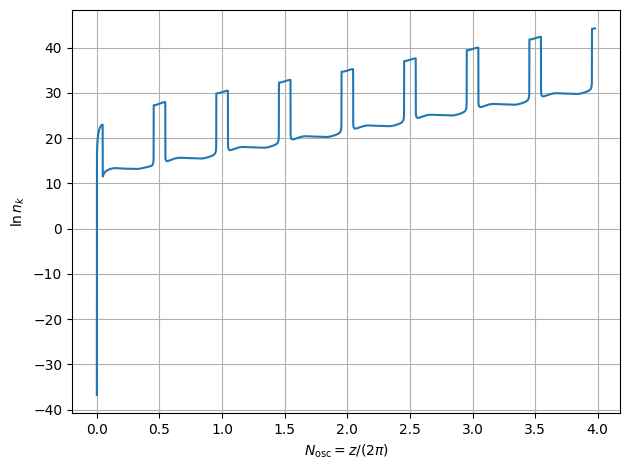
\includegraphics[width=300pt]{images/particle production phi.png}
% \end{center}

\selectlanguage{english}
\begin{figure}[H]
    \centering
    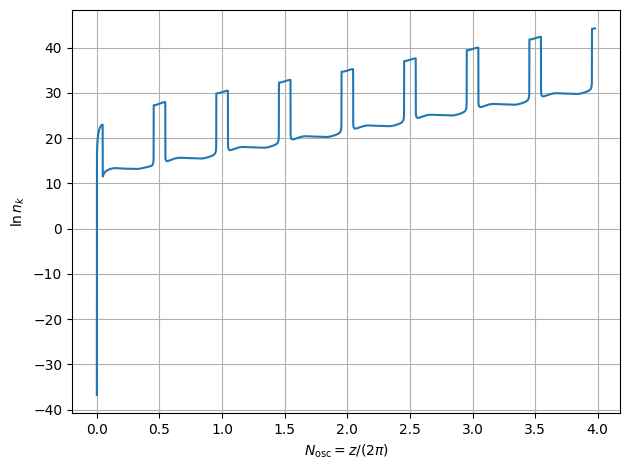
\includegraphics[width=300pt]{images/particle production phi.png}
    \caption{Comoving particle production indicator $\ln n_k$ obtained numerically in this work during the evolution of the inflaton-only system. The step-like increase with intermediate jumps is a coordinate artifact of using comoving variables; a more physical treatment including the coupled $\chi$ and $\theta$ fields would introduce backreaction and effective friction, modifying both the inflaton evolution and particle production rate.}
    \label{fig:particle_production_phi}
\end{figure}

Here we can notice a slight difference to the previous results, it is that the number of particles seems to be growing monotonically with jump-like intermediate behaviour. This, again is the consequence of the choice of coordinates. The computation of the particle number would obviously change with the introduction of $\chi$ and $\theta$. These fields would act as friction, limiting the growth of $\phi$, by converting the inflaton field energy into particle production. Note however, that the coupling is non-trivial, so further investigation must be done.

It should be noted that the numerical results presented here are just a simplified background evolution where the inflaton is evolved independently by taking $\langle \chi \rangle=\langle \theta \rangle=0$. While this approximation is sufficient for capturing the inflationary stage and determining $N_{\rm end}$, it neglects the most important reheating effects: energy transfer from $\phi$ into matter degrees of freedom, backreaction on the inflaton dynamics, and the emergence of an effective friction term sourced by particle production. Consequently, the post-inflationary evolution in the inflaton-only system is not expected to be physically realistic, since $\phi$ does not dissipate energy and its growth remains unbounded. Furthermore, the occupation number $n_k$ computed in comoving variables can exhibit non-monotonic behaviour which depends on the choice of coordinates and on the definition of the instantaneous frequency $\omega_k(t)$. Further work is required to include the $\chi$ and $\theta$ evolutions, together with the averages and PI corrections.

% \section*{Conclusions}

% \begin{itemize}
%     \item Equations of motion for the $V(\phi) = V_0 \exp ( - \kappa \exp(\frac{\phi}{b M_{\rm pl}})) $ were investigated
%     \item Numberical integrator was written using fourth order Runge-Kutta algorithm. With an algorithm for investigation of inflaton field
%     \item Simulations of the inflaton field equation of motion compute the end of inflation, inflaton field evolution, which concide with the slow-roll and kination limits.
% \end{itemize}

\section*{Conclusions}

In this work the equations of motion for the inflationary potential
$V(\phi)=V_0 \exp\!\left[-\kappa \exp\!\left(\frac{\phi}{b M_{\rm Pl}}\right)\right]$ were investigated. A numerical integrator was implemented using the fourth-order Runge--Kutta (RK4) algorithm, which was then used to study the evolution of the inflaton field. The simulations allowed us to compute the inflaton field trajectory and determine the end of inflation, and the obtained results are consistent with the expected behaviour in the slow-roll and kination limits. Finally, many results from \cite{kofman1997towards} were reproduces, using numerical simulations. 


\addcontentsline{toc}{section}{Conclusions}


\addcontentsline{toc}{section}{References}\bibliographystyle{BibStyle}
\bibliography{Bibliography}


\end{document}
